In order to eliminate the Chainsewing Attack we propose an update to the velvet
NIPoPoW protocol. The core problem is that in her suffix proof the adversary
is able to claim not only blocks of a forked chain,  which are in majority adversarially
generated due to the Common Prefix property, but also an arbitrarily long part of the
chain adopted by an honest player. Since thorny blocks are accepted as valid,
the verifier cannot distinguish blocks that actually belong in a chain from
blocks that only seem to belong in the same chain because they are pointed to
via a non-smooth pointer. \\

We will first define our security assumptions and then discuss some solution
approaches for the problem. This discussion will result to the proposed protocol
upgrade suggestion.

\subsubsection{Velvet fork parameter}
Under stable conditions a velvet fork suggest that only a minority of upgraded parties needs to support the protocol update. Let $g$ express the percentage of honest upgraded parties to the total number of miners. We will refer to $g$ as the ``velvet parameter".

\begin{defn}{\textbf{Velvet Parameter}}
	\textit{Let $g$ be the velvet parameter for NIPoPoW protocols.  Then if $n_h$ the upgraded honest miners and $n$ the total number of miners it holds that $n_h = g \cdot n$.}
	\label{defn:velvet_honest_majority}
\end{defn}

%% first reference to 1/3 adversary
\subsubsection{Honest Majority Assumption}
Compared to the typical setting of $1/2$-bounded adversary, the protocol we
propose requires stronger honest majority assumptions to be provably secure. 
In particular, our protocol is secure for adversary of total hashing power 
less than $1/3$ of the upgraded honest miners. Therefore we define the Velvet
Honest Majority assumption, which will be used in our security proof.

\begin{defn}{\textbf{Velvet Honest Majority}}
	\textit{Let $n_v$ be the number of upgraded miners. Then $t$ out of total $n_v$
	parties are corrupted such that $\dfrac{t}{n_v} < \dfrac{1 - \delta}{3} $. }
	\label{defn:velvet_honest_majority}
\end{defn}
We believe that if we waive this requirement it is impossible to have a provably 
secure NIPoPoW protocol under velvet fork conditions.
This claim is described and discussed in the following.
Note that any reference to adversarial party bound is respect to the number of
upgraded parties $n_v$. Therefore, ``(1/2)-bounded adversary" holds for
$\dfrac{t}{n_v} < \dfrac{1 - \delta}{2} $, while ``(1/3)-bounded adversary" holds for
$\dfrac{t}{n_v} < \dfrac{1 - \delta}{3} $.

\subsubsection{Impossibility of a secure protocol for (1/2)-bounded adversary}
During our study on the problem we failed to prove the security of several protocol
constructions under $(\frac{1}{2})$-bounded adversary. We finally concluded that
such a secure NIPoPoW construction is impossible under velvet fork conditions.
Though it is hard to provide a typical proof for this claim, as one should consider
any possible construction, we try to argue for it in this section.

\textbf{Claim:} \textit{Assume $t$ adversarial out of total $n_v$ upgraded parties.
There is no construction for NIPoPoW suffix proofs under velvet fork conditions,
which is both succinct and secure for every adversary, such that
$\dfrac{t}{n_v} < \dfrac{1 - \delta}{2} $.}

\textit{Discussion.} As explained earlier, since the adversary may use the interlink
structure so as to include pointers to arbitrary blocks,  she may construct her own
chain history utilizing the non-smooth pointers included in the thorny blocks she
generates. Such an example is given in Figure \ref{fig:generic_attack}.

Let us consider a protocol construction $p$ which allows for NIPoPoW suffix proofs
under velvet fork and is secure for 1/2-bounded adversary. Our main
goals are $p$ to be both secure and succinct. We can even loose our non-interactivity
limitations to make it possible to challenge the submitted proofs, so that an honest
player can contest against an inconsistent proof. However, note that the same power
to challenge any submitted proof is also provided to the adversary.

Now assume an adversary of $ n_v/3 < t < n_v/2 $. Then, as explained
in the Backbone and Selfish Mining papers \cite{Backbone}\cite{selfish_mining} it
is possible for the adversary to maintain the longest valid chain being of less
than $50\%$ chain quality in favor of adversarially generated blocks. In particular,
consider that the adversary mines selfish, meaning that for every block she mines
she does not immediately announce it to the network. Instead, she waits until an
honest block is announced. In the worst case, consider an adversary that has a
network advantage regarding the relay of her blocks. Thus in case of two competing
blocks in a round the adversarial one will be appended to the chain, while the
honest block is discarded in practice as a temporary fork. Because of this attack
the total block ratio in the chain will result as illustrated in Figure
\ref{fig:selfish_mining_pie}. For (1/3) adversary half of the blocks in the
chain are expected to be adversarial, while for (1/2) adversary no honest block
is included in the chain in the worst case scenario.

\begin{figure}[h!]
	\begin{center}
		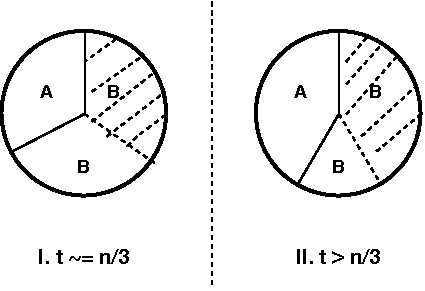
\includegraphics[scale=0.8]{figures/selfish_mining_pie.pdf}
	\end{center}
	\caption{\textit{Pie chart of adversarially and honestly generated blocks appended in 
	the chain during a round set S. Part \textbf{A} stands for blocks mined by the
	adversary while \textbf{B} for blocks mined by honest players. Lined out parts
	denote honestly mined blocks that were defeated by adversarially mined ones in
	the same round due to selfish mining.\textbf{I.} With $t = n/3$, $50\%$ of the
	total blocks are adversarially generated in the worst case scenario. \textbf{II.}
	With $t > n/3$, more than half of the total blocks are adversarially generated in
	the worst case scenario.}}
	\label{fig:selfish_mining_pie}
\end{figure}

Observe that the property violated in the chainsewing attack is the $prevId$ relation
between sequential blocks. However since the main purpose of our work is to achieve
succinctness, the \textit{prevId} relations could not be utilized in a viable manner
in order to contest adversarial proofs, as it would require proofs of linear length
to that of the whole chain.  We thus conclude that we should mostly rely on the
information given by the interlink pointers as far as the validity of any proof
is concerned so as to keep our protocol construction efficient.

Now assume, to honest parties' favor, that it is both possible and efficient to inspect
the whole chain history that each block is commited to via its interlink pointers. Keep
in mind that an adversary can keep a consistent chain considering the interlink pointers
by using only her own mined blocks and, at the same time, these blocks may overwhelm
the honestly generated ones. In our protocol $p$ it should be decided  under what policy
an honest party generates blocks and constructs suffix proofs. A decision should be made
for block generation:
\begin{enumerate}
\item interlink data are neutral as for adversarially and honestly generated blocks
\item interlink data point out inconsistent blocks, meaning blocks with incorrect
interlinks\item interlink data exclude inconsistent blocks from being part of the
valid chain formed by the super-pointers
\end{enumerate}
Now let's examine the above choices. \\
In the first case the arguments that an honest player could provide against an
inconsistent proof could only be based on the 0-level pointers. Such a contesting
proof should at least provide the 0-level subchain of length equal to the
following: starting from a block included in the suffix proof and is not a
block of the chain until the closest block included in the suffix proof and is
a valid block of the chain. This means that contesting proofs are expected to
be of length $2^\mu$ where $\mu = log(|C|)$, and subsequently are of complexity
$\mathcal{O}(|C|)$ which ruins the succinctness of our protocol.

In the second case an honest party could utilize this extra information provided
in the interlink to prove an inconsistent proof wrong. However, keep in mind that
the adversary could make such claims too. So, a claim of inconsistency for a
specific block included should be followed by a proof of its inconsistency.
Whatever the information considering the incorrect blocks in the interlink may
be, the adversary could make some of it in her own generated blocks in order to
contest an honest proof too. So we fall to the previous case turning to
\textit{prevId} pointers in order to prove the true chain history, where the
contesting proofs are unacceptable efficiency-wise.

In the third case we demand from the honest players to validate the interlink
structures of the blocks in the chain and exclude the inconsistent ones from
the chain history that the interlinks provide. In this way we could possibly
provide contesting proofs using information only from the interlinks thus
keeping our proofs succinct. This solution would result to two different
chain histories considering the interlink pointers: the one of the honest
parties that includes only blocks with valid interlinks, and the one of the
adversary which may form her own history of invalid blocks probably belonging
to many different underlying chains but could not include honest blocks if at
least one invalid block participates in the proof. This solution seems to bring
us to a notable trade-off point. On the one hand we manage to uncouple from the
0-level blocks. On the other hand, we compromise that honest players cannot use
valid adversarially generated blocks in their proof, while the adversary cannot
include honestly generated blocks in her proofs if inconsistent blocks are also
included. This solution could not work properly for (1/2)-bounded adversary
though. The reason lies in the bad chain quality as pointed out earlier and shown in
Figure \ref{fig:selfish_mining_pie}. If the adversary  could create his own chain
history including inconsistent blocks from two different chains, then she could
easily construct a suffix proof that wins over an honest one because the majority
of the blocks included in the chain could be adversarial with high probability.

We conclude that such a protocol could not exist for (1/2)-bounded adversary.


\subsubsection{Solution for (1/3)-bounded adversary}
The vulnerability that makes this attack possible is the acceptance of thorny
blocks. Since we operate under a velvet fork we cannot eliminate such blocks, 
but we need, however, to restrict the adversary from being able to claim portion
of another chain as part of her own fork chain.The key observation on the
Chainsewing Attack is that the adversary needs at least one adversarially generated
block in an honest player's chain (block $a'$), in order to create a path of
superpointers connecting blocks of two, or more, diverse chains. The final proof
chain will make use of this crossing point and may contain both honest or
adversarial blocks.
%% intuitive reference to 1/3 adversary
In case the proof contains only adversarial blocks, the attack cannot harm
security for an adversary of less than $1/3$ of the total hashing power. This
fact will be clear in the security proof section. In short, as argued in the
previous section an adversary of $1/3$ of the total hashing power may contribute
at most $ 50\% $ of the total blocks in the longest valid chain. An attacker of
more than $1/3$ hashing power could dominate as of total hashing power expressed
in mined blocks in the chain, while the inverse would be true for an attacker of
less hashing power than this threshold.

So in order to be successful, the attacker needs to also ``sew`` honestly generated
blocks. Thus there will be at least one honest block in the superblock path which
connects $a$ and $a'$, pointing to an adversarial thorny block.

The idea is to ban all blocks generated by honest players from participating in
this superblock path. In this way the adversary could not misuse hashing power of
the honest players and the sewed blocks could only be adversarially generated,
thus the attack could never succeed for an adversary of less than $1/3$ of the
total hashing power.

We describe a protocol patch that operates as follows. The NIPoPoW protocol under
velvet fork works as usual but each miner constructs smooth blocks. This means
that  a block's interlink is constructed excluding thorny blocks (except the
pointers of level 0). In this way, although thorny blocks are accepted in the
chain, they are not taken into consideration when updating the interlink structure
for the next block to be mined. No honest block could now point to a thorny superblock
that may act as the passing point to the fork chain in an adversarial suffix proof.
Thus, after this protocol update the adversary is only able to inject adversarially
generated blocks from the chain adopted by an honest party to her own fork.
At the same time, thorny blocks cannot participate in an honestly
generated suffix proof except for some blocks in the proof's suffix $(\chi)$.
This arguments holds because thorny blocks do not form a valid chain along with
honestly mined blocks anymore. Consequently, as far as the blocks included in a
suffix proof is concerned, we can think of thorny blocks as belonging in the
adversary's fork chain for the $\pi$ part of the proof,  which is the comparing
part between proofs. Figure \ref{fig:injection} illustrates this remark.\\

\begin{figure}[h!]
	\begin{center}
		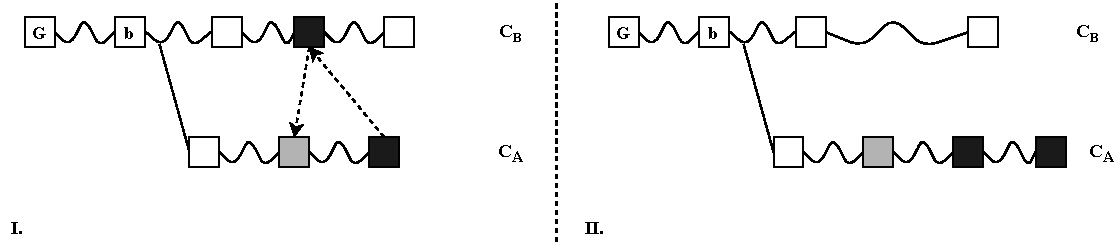
\includegraphics[scale=0.5]{figures/injection.png}
	\end{center}
	\caption{\textit{The adversarial fork chain $C_A$ and chain $C_B$ of an honest
	player. Thorny blocks are colored black. Dashed arrows represent interlink
	pointers. Wavy lines imply one or more blocks. When an adversarially generated
	block is sewed from $C_B$ into the adversary's suffix proof the verifier
	conceives $C_A$ as longer and $C_B$ as shorter.  \textbf{I:} The real picture
	of the chains. \textbf{II:} Equivalent picture from the verifier's perspective
	considering the blocks included in the corresponding suffix proof for each chain.}}
	\label{fig:injection}
\end{figure}


The protocol patch we suggest can be summarized as follows:\\


\subsubsection*{Protocol Patch for NIPoPows suffix proofs under velvet fork.} In order
to make NIPoPoWs safe under velvet fork conditions we suggest:
\begin{enumerate}
\item Strengthen the Honest Majority Assumption so that $2t < (1 - \delta)(n_v-t)$,
where $n_v$ is the number of upgraded players.
%%% TODO: also provide short algorithm for the intrlink construction after the patch 
\item The NIPoPoW protocol under velvet fork works as usual but a miner constructs
a block's interlink without pointers to thorny blocks.
\end{enumerate}

The following Lemmas come as immediate results from the suggested protocol
update.\\

\begin{lemma}
	\textit{A velvet suffix proof constructed by an honest player cannot contain
	any thorny block.}
	\label{lemm:smooth_honest_suffix}
\end{lemma}

\begin{lemma} 
	\textit{Let $\mathcal{P_A} = (\pi_\mathcal{A}, \chi_\mathcal{A})$
	be a velvet suffix proof constructed by the adversary and block $b_s$, generated
	at round $r_s$, be the most recent smooth block in the proof. Then $\forall r:r < r_s$ no thorny blocks generated at round $r$ can be included in $\mathcal{P_A}$.}
	\label{lemm:smooths_before_smooth}
\end{lemma}
\textit{Proof.} By contradiction. Let $b_t$ be a thorny block generated at
some round $r_t < r_s$. Suppose for contradiction that $b_t$ is included in
the proof. Then, because $\mathcal{P_A}$ is a valid chain as for interlink
pointers, there exist a block path made by interlink pointers starting from $b_s$
and resulting to $b_t$. Let $b'$ be the most recently generated thorny block
after $b_t$ and before $b_s$ included in $\mathcal{P_A}$. 
Then $b'$ has been generated at a round $r'$ such that $r_t \leq r' < r_s$. Then
the block right after block $b'$ in $\mathcal{P_A}$ must be a thorny block since
it points to $b'$ which is thorny. But $b'$ is the most recent thorny block after
$b_t$, thus we have reached a contradiction.
\begin{flushright}
$\square$
\end{flushright}

\begin{lemma}
	\textit{Let $\mathcal{P_A} = (\pi_\mathcal{A}, \chi_\mathcal{A})$
	be a velvet suffix proof constructed by the adversary. Let $b_t$ be the oldest
	thorny bock included in $\mathcal{P_A}$ which is generated at round $r_t$. Then any block $b = \{b: b \in \mathcal{P_A} \wedge \text{b generated at }r \geq r_t \}$ is thorny.}
	\label{lemm:thorny_after_thorny}
\end{lemma}
\textit{Proof.} By contradiction. Suppose for contradiciton that $b_s$ is a smooth block generated at round $r_s > r_t$. Then from Lemma \ref{lemm:smooths_before_smooth} any block generated at round $r < r_s$ is smooth. But $b_t$ is generated at round $r_t < r_s$ and is thorny, thus we have reached a contradiction.
\begin{flushright}
$\square$
\end{flushright}

The following corollary emerges immediately from Lemmas \ref{lemm:smooths_before_smooth}, \ref{lemm:thorny_after_thorny}. This result is illustrated in Figure \ref{fig:adversarial_velvet_proof}.

\begin{corollary}
	\textit{Any adversarial proof $\mathcal{P_A} = (\pi_\mathcal{A}, \chi_\mathcal{A})$, containing both smooth and thorny blocks, consists of a prefix smooth subchain followed by a suffix thorny subchain.}
	\label{cor:adversarial_proof_scheme}
\end{corollary}

\begin{figure}[h!]
	\begin{center}
		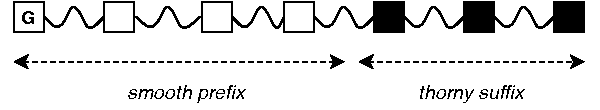
\includegraphics[scale=0.75]{figures/adversarial_velvet_proof.pdf}
	\end{center}
	\caption{\textit{In the general case the adversarial velvet suffix proof $\mathcal{P_A} = (\pi_\mathcal{A}, \chi_\mathcal{A})$ consists of an initial part of smooth blocks followed by  of thorny blocks.}}
	\label{fig:adversarial_velvet_proof}
\end{figure}

We now describe the algorithms needed by the upgraded miner, prover and verifier. The upgraded miner acts as usual except for including the interlink of the newborn block in the coinbase transaction. In order to construct an interlink containing only the smooth blocks, the miner keeps a copy of the ``smooth chain'' ($\mathcal{C}_S$) which consists of the smooth blocks existing in the original chain $\mathcal{C}$. The algorithm for extracting the smooth chain out of $\mathcal{C}$ is given in Algorithm \ref{alg:smooth_chain}. Function \textit{isSmoothBlock(B)} checks whether a
block \textit{B} is a smooth velvet by calling \textit{isSmoothPointer(B,p)}
for every pointer \textit{p} in \textit{B}'s interlink. Function
\textit{isSmoothPointer(B,p)} returns \emph{true} if $p$ is a valid 
pointer, in essence a pointer to the most recent \emph{smooth velvet}
for the level denoted by the pointer itself. The \textit{updateInterlink} algorithm is given in Algorithm \ref{alg:updateInterlink}, which is essentially the same as in the case of a hard/soft fork, except for working on the smooth chain $\mathcal{C}_S$ instead of $\mathcal{C}$.

\begin{algorithm}[H]
	\SetAlgoNoLine
	\DontPrintSemicolon
	\SetKwProg{Fn}{function}{:}{\text{end function}}
	\Fn{smoothChain($\mathcal{C}$)}{
		$\mathcal{C}_S = \{ \mathcal{G} \}$\;
		$k \leftarrow 1$ \;
		\While{$\mathcal{C}[-k] \neq \mathcal{G}$}{
			\If{isSmoothBlock($\mathcal{C}[-k]$)}{
				$\mathcal{C}_S \leftarrow \mathcal{C}_S \cup \mathcal{C}[-k]$\;
			}
			$k \leftarrow k + 1$\;
		}
		return $\mathcal{C}_S$
	}
	\vspace{4mm}
	\Fn{isSmoothBlock(B)}{
		\If{$B = \mathcal{G}$}{
			\Return true\;
		}
 		\For{p $\in$ B.interlink} {
     		\If{$\neg$isSmoothPointer(B, p)}{
     			\Return false\;
     		}
 		}
 		\Return true\;
	}
	\vspace{4mm}
	\Fn{isSmoothPointer(B, p)}{
		$b \leftarrow Block(B.prevId)$\;
 		\While{b $\not =$ p} {
     		\If{$ level(b) \geq level(p) \wedge
     			\text{isSmoothBlock(b)} $}{
     			\Return false\;
     		}
     		\If{$b = \mathcal{G}$}{
     			\Return false\;
     		}
     		$b \leftarrow Block(b.prevId)$
 		}
		 \Return $\textit{isSmoothBlock(b)}$ \;
	}
 	\caption{Compute smooth chain}
 	\label{alg:smooth_chain}
\end{algorithm}

\begin{algorithm}[h!]
	\SetAlgoNoLine
	\DontPrintSemicolon
	\SetKwProg{Fn}{function}{:}{\text{end function}}
	\Fn{updateInterlinkVelvet($\mathcal{C}_S$)}{
		B' $\leftarrow \mathcal{C}_S[-1]$\;
		interlink $\leftarrow$ B'.interlink\;
 		\For{$\mu = 0$ to level(B')}{
 			interlink$[\mu]\leftarrow id(B')$
		 }
 		\Return interlink\;
	}
 	\caption{Velvet updateInterlink}
 	\label{alg:updateInterlink}
\end{algorithm}

The construction of the velvet suffix prover is given in Algorithm \ref{alg:velvet_suffix_prover}, which is essentially the same to that of a hard/soft fork except for working on smooth chain $\mathcal{C}_S$ instead of $\mathcal{C}$.

\begin{algorithm}[h!]
	\SetAlgoNoLine
	\DontPrintSemicolon
	\SetKwProg{Fn}{function}{:}{\text{end function}}
	\Fn{$ProveVelvet_{m,k}(\mathcal{C}_S$)}{
		$B \leftarrow \mathcal{C}_S[0]$\;
		\For{$\mu = \vert \mathcal{C}_S[-k].interlink \vert$ down to 0}{
			$\alpha \leftarrow \mathcal{C}_S[:-k] \{ B: \} \uparrow^\mu$\;
			$\pi \leftarrow \pi \cup \alpha$\;
			$B \leftarrow \alpha[-m]$\;
		}
		$\chi \leftarrow \mathcal{C}_S[-k:]$\;
		\Return $\pi\chi$
	}
 	\caption{Velvet Suffix Prover}
 	\label{alg:velvet_suffix_prover}
\end{algorithm}

\vspace{4mm}

In conclusion the Verify algorithm for the NIPoPoW suffix protocol remains the same as in the case of hard or soft fork.